\documentclass[11pt,]{article}
\usepackage[margin=1in]{geometry}
\newcommand*{\authorfont}{\fontfamily{phv}\selectfont}
\usepackage[]{mathpazo}
\usepackage{multicol}
\usepackage{abstract}
\renewcommand{\abstractname}{}    % clear the title
\renewcommand{\absnamepos}{empty} % originally center
\newcommand{\blankline}{\quad\pagebreak[2]}

\providecommand{\tightlist}{%
  \setlength{\itemsep}{0pt}\setlength{\parskip}{0pt}} 
\usepackage{longtable,booktabs}
      
\usepackage{parskip}
\usepackage{titlesec}
\titlespacing\section{0pt}{12pt plus 4pt minus 2pt}{6pt plus 2pt minus 2pt}
\titlespacing\subsection{0pt}{12pt plus 4pt minus 2pt}{6pt plus 2pt minus 2pt}

\titleformat*{\subsubsection}{\normalsize\itshape}

\usepackage{titling}
\setlength{\droptitle}{-.15cm}

%\setlength{\parindent}{0pt}
%\setlength{\parskip}{6pt plus 2pt minus 1pt}
%\setlength{\emergencystretch}{3em}  % prevent overfull lines 

\usepackage[T1]{fontenc}
\usepackage[utf8]{inputenc}

\usepackage{fancyhdr}
\pagestyle{fancy}
\usepackage{lastpage}
\renewcommand{\headrulewidth}{0.3pt}
\renewcommand{\footrulewidth}{0.0pt} 
\lhead{}
\chead{}
\rhead{\footnotesize BUS 1301: Managing with Data, Analytics, and
Artificial Intelligence -- Spring 2026}
\lfoot{}
\cfoot{\small \thepage /\pageref*{LastPage}}
\rfoot{}

\fancypagestyle{firststyle}
{
\renewcommand{\headrulewidth}{0pt}%
   \fancyhf{}
   \fancyfoot[C]{\small \thepage/\pageref*{LastPage}}
}

%\def\labelitemi{--}
%\usepackage{enumitem}
%\setitemize[0]{leftmargin=25pt}
%\setenumerate[0]{leftmargin=25pt}




\makeatletter
\@ifpackageloaded{hyperref}{}{%
\ifxetex
  \usepackage[setpagesize=false, % page size defined by xetex
              unicode=false, % unicode breaks when used with xetex
              xetex]{hyperref}
\else
  \usepackage[unicode=true]{hyperref}
\fi
}
\@ifpackageloaded{color}{
    \PassOptionsToPackage{usenames,dvipsnames}{color}
}{%
    \usepackage[usenames,dvipsnames]{color}
}
\makeatother
\hypersetup{breaklinks=true,
            bookmarks=true,
            pdfauthor={},
             pdfkeywords = {},  
            pdftitle={BUS 1301: Managing with Data, Analytics, and
Artificial Intelligence},
            colorlinks=true,
            citecolor=blue,
            urlcolor=blue,
            linkcolor=magenta,
            pdfborder={0 0 0}}
\urlstyle{same}  % don't use monospace font for urls


\setcounter{secnumdepth}{0}

\usepackage{longtable}

\usepackage{graphicx}
% We will generate all images so they have a width \maxwidth. This means
% that they will get their normal width if they fit onto the page, but
% are scaled down if they would overflow the margins.
\makeatletter
\def\maxwidth{\ifdim\Gin@nat@width>\linewidth\linewidth
\else\Gin@nat@width\fi}
\makeatother
\let\Oldincludegraphics\includegraphics
\renewcommand{\includegraphics}[1]{\Oldincludegraphics[width=\maxwidth]{#1}}



\usepackage{setspace}

\title{BUS 1301: Managing with Data, Analytics, and Artificial
Intelligence}
\date{Spring 2026}


\begin{document}  

		\maketitle
		
	
		\thispagestyle{firststyle}

%	\thispagestyle{empty}
\textbf{\underline{Instructor}}
\begin{multicols}{2}

  \textbf{Robert W. Walker, Ph. D.}\\
  Email: \href{mailto:rwalker@willamette.edu}{\nolinkurl{rwalker@willamette.edu}}\\
  Preferred contact: Email\\
  Office Hours: 13:30-14:30 p.m. TTh\\
  Office: Kaneko 208, Salem\\
  Correspondence policy: Within 24 hours on weekdays; 48 hours on
weekends\\
    \columnbreak
    
  \end{multicols}
	
\noindent \begin{tabular*}{\textwidth}{ @{\extracolsep{\fill}} lr @{\extracolsep{\fill}}}
\textbf{\underline{Class information}}\\
  Classroom: Kaneko 120\\
  Class Hours: 14:50 - 16:20 pm TTh\\
    \\
	\end{tabular*}\\


\vspace{2mm}


\subsection{Course description}\label{course-description}

This course will introduce students to how managers and organizations
collect, process, and interpret observations about the world around them
to facilitate informed decisions with the aid of models including those
of artificial intelligence. The first portion of the course introduces
students to models, the concept of data, and the use of data in
workplace settings. Students will learn different practical methods of
data gathering -- from surveys and archives to experiments and crowd
sourcing and explore basic methods of organizing data for robust and
sustainable deployment. With data in hand, we explore how managers can
use data, highlighting the incredible value resulting from cross
tabulation, frequency distributions, and simple plots. This value is
enhanced with basic statistical inference and populating models with
data. One of the greatest barriers to linking data and decisions was the
necessary computing; artificial intelligence tools have fundamentally
changed that. The final portion of the course will focus on the use of
artificial intelligence (AI), highlighting general features of how
commonly deployed AI systems function and how they can solve challenges
across various areas of business and explore the likely future.

Information is a resource; it should be used judiciously and
efficiently. While a wealth of information is available at our
fingertips, high quality information can remain a surprisingly scarce
resource. We are inundated with data, facts, and figures that only
become actionable through identifying meaningful patterns and trends,
developing fundamental managerial insights, and extracting information
essential to inform effective managerial decisions. The tools of this
course are among the most important tools of effective managers.

While effective, there is a sense in which limitations imposed by
linking decisions to measures and data are reductionist, potentially
misleading, and pose potentially deep ethical challenges. Mindful of the
central role that ethics must play in shaping organizational pursuits,
we will tackle these challenges head on though only you can ground these
in your deepest moral sentiments.

\section{Course goals}\label{course-goals}

Upon successful completion of this course, you should --

\begin{enumerate}
\def\labelenumi{\arabic{enumi}.}
\tightlist
\item
  Distinguish various means of data collection and discuss their
  tradeoffs.
\item
  Describe common models of data management and their tradeoffs.
\item
  Understand the basics of relational databases and the ways that they
  are combined.
\item
  Articulate the application of common analytic techniques, their
  function, and their domain of application.
\item
  Comfortably discuss AI's historical development, current
  functionality, and valid use cases.
\item
  Recognize and evaluate the myriad ethical concerns in data, analytics,
  and artificial intelligence.
\item
  Be able to utilize AI tools {[}and verify their veracity{]} for
  performing data analysis and decision support.
\end{enumerate}

\section{Course Materials}\label{course-materials}

The primary organizing resource for the course is the \textbf{Open
Introduction to Statistics}. It is open and freely available in a
variety of digital formats. Paper copies can be obtained as well if you
so choose.

\begin{verbatim}
Diez, David M., Christopher D. Barr, and Mine Cetinkaya-Rundel.  2019.  
  OpenIntro Statistics: Fourth Edition.
\end{verbatim}

Additional course materials -- readings, examples, and exercises -- will
be posted regularly to our Canvas course site and the class website. I
maintain Files and a Pages document with .pdfs and links on Canvas and
will frequently link things via the course website on github.

To access the university sites, you will be prompted for your Willamette
University login in order to gain access to course materials. The course
will combine the use of Excel or Sheets for many tasks but we have
reached an age where what once were difficult computing barriers have
become trivial for LLM tools. We will exploit them.

Slides are always posted before class. Supplemental resources can be
found on Canvas.

\section{Policies}\label{policies}

\subsection{Individuals and Groups}\label{individuals-and-groups}

This course will require you to complete both individual assignments and
group assignments. For individual assignments, I do not allow any form
of student collaboration. I define student collaboration as any
assistance given from one student to another student. Please feel free
to talk with me before you engage in any activity that might satisfy the
definition of ``collaboration''; I would be happy to provide you my
guidance on whether or not the activity is acceptable. By enrolling in
this course, you agree to be held to my definition of ``individual
assignments'' and ``student collaboration.'' For group assignments,
students can and should work interactively, making it difficult to
distinguish who completed which portions of the project. In the list of
deliverables below, I designate individual work and group work.

\subsection{AI Tools and Their Use}\label{ai-tools-and-their-use}

Exams with integrity are a challenge. I am not restricting use of AI
tools at all for your exam prep memos or for class exercises. However,
you must keep two things in mind: using an AI system does not absolve
you from the need to cite others' work and you have to verify any
information that an AI system provides. You will receive point
deductions for uncited or incorrect information, as well as for uncited
incorrect information (the latter sounds strange, but it can happen if
you echo someone else's erroneous ideas). You also must disclose when
you use AI in your work; this disclosure should not be viewed as a
hassle, but, instead, as an opportunity to display your skill in using
AI systems. If you do find yourself thinking that the use of an AI
system for a given activity is something you would rather not disclose,
then I would contend that you do not need any further evidence to
realize that you ought to dispense with the use of AI in that situation:
just do the work on your own.

\subsection{Holidays and Absence}\label{holidays-and-absence}

The academic calendar spans religious holidays, days of personal
obligation, exceptional one-time work situations, bouts of illness, and
unexpected difficult incidents that change our lives, such as the loss
of family members or friends. If one of those important events (or any
other important circumstance not listed) occurs on or near a day when we
have a class session or deliverable due, please contact me. Together we
will figure out an alternative arrangement that allows you to complete
the requirements of this course without penalty while maintaining focus
on important things that require personal attention. If you face a
particularly severe situation that will require you to miss many class
sessions, please contact me so that we can work together to determine
whether it makes sense for you to step away from the course and complete
it in the future, thus avoiding an additional stressor in the midst of
exceptional challenges. In any event, please know that I firmly believe
in accommodating every student's important religious and personal
commitments.

\subsection{Attendance policy}\label{attendance-policy}

\begin{itemize}
\tightlist
\item
  Because \texttt{google\ meet} recordings of every course meeting are
  available, there are opportunities for making up missed classes; I
  take this as license to assume you are familiar with the complete
  contents of every class meeting. It is not a substitute for attentive
  and active presence. It is an opportunity not to miss things.
\end{itemize}

The university views this course as \texttt{in-person}. Students cannot
complete class exercises remotely, however, thus those attending
remotely will need to schedule a meeting with me to complete the
exercise.

\pandocbounded{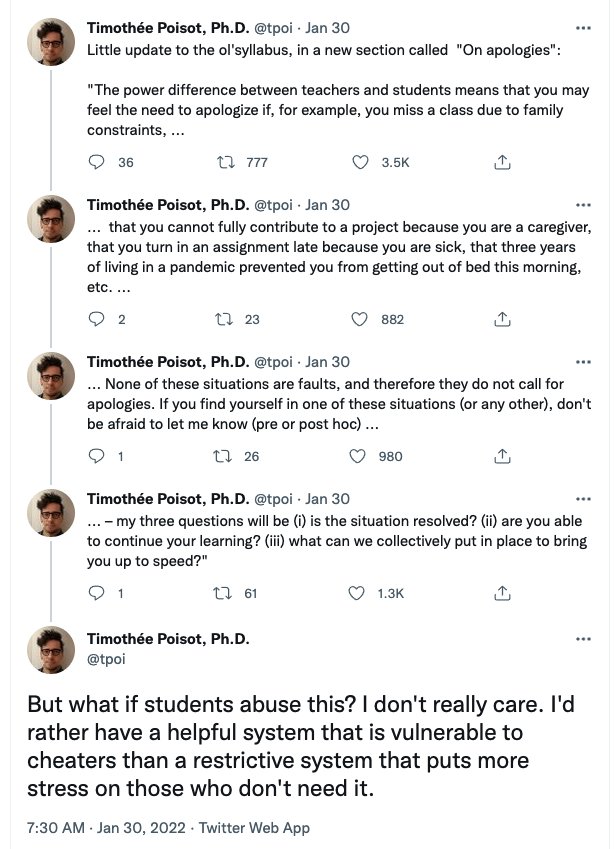
\includegraphics[keepaspectratio]{unknown.png}}

\section{Grading}\label{grading}

\begin{longtable}[]{@{}lr@{}}
\toprule\noalign{}
Grade & Range \\
\midrule\noalign{}
\endhead
\bottomrule\noalign{}
\endlastfoot
A & 95-100 \\
A- & 90-94.5 \\
B+ & 85-89.5 \\
B & 80-84.5 \\
B- & 75-79.5 \\
C & 70-74.5 \\
C- & 65-69.5 \\
D+ & 60-64.5 \\
D & 55-59.5 \\
F & 0-54.5 \\
\end{longtable}

\textbf{I am not 100 percent certain on this part, we will discuss it.}

\begin{itemize}
\item Some Submission During Class Time (20 points for 20 meetings)
\item Class Exercises (180 points). To engage with our course readings and concepts thoroughly, the course will involve exercises in nearly every class session. The scores from your top 18 exercises will be counted in your course grade. Class exercises will involve tasks that reinforce concepts in the reading and class session.  In many cases, these must be done **during class** so attendance is crucial.  Students receive a baseline of 6 points for submitting the exercise and the remaining 4 points are performance based. [Mix of individual and group work.]
\item Cases (100 points) Extended exercises spanning multiple discrete days of instructions highlighting a management problem and providing multi-part solutions.  [Mix of individual and group work]
\item Exam Prep Memos (100 points). To prepare for the course’s exams, students must draft a memo in which they identify important course concepts and provide an example of each concept. All work will take place in class and guidance will be provided in the review sessions. [Mix of individual and group work.]
\item Midterm Exam (150 points). The course will include a midterm exam covering the first half of the semester. Exam items will include multiple choice and short answer questions. [Individual work]
\item Final Exam (150 points). The course will include a final exam covering the second half of the semester. [Individual Work]
\end{itemize}

\subsection{Willamette Code of
Conduct}\label{willamette-code-of-conduct}

Every student is expected at all times to abide by the Willamette
University Atkinson Graduate School of Management Honor Code, Academic
Integrity Policy, and Expectations of Academic and Professional Behavior
as detailed in the current student handbook:
\url{https://willamette.edu/mba/students/full-time/mba-student-handbook/index.html}

College of Arts and Sciences
\url{https://my.willamette.edu/site/policies/academic-integrity}

\subsection{Diversity and Inclusion
Statement:}\label{diversity-and-inclusion-statement}

I intend for students from all backgrounds and perspectives to be well
served by this course. The Diversity of thought and experience that
everyone brings to this class should be viewed as a resource, strength,
and benefit. As such, we will strive to be open-minded and understanding
of everyone's perspectives and polite to each other when we disagree.

\section{Class Recordings}\label{class-recordings}

I will do my very best to insure useful \texttt{google\ meet} recodings
for every class. They are accessible via Canvas.

\section{Solicitation of Input}\label{solicitation-of-input}

Student input for the purpose of course improvement is taken very
seriously and will potentially be done periodically. Please take the
time to evaluate this course and the instructor, especially at the end
of the semester. Evaluations will in no way affect your grade. I simply
cannot know the student experience in the classroom without your
perspective.

\subsection{Campus Weather Closure}\label{campus-weather-closure}

In case of extreme weather conditions or when the university is closed,
classes are expected to be fully on \texttt{google\ meet}. Unless the
instructor makes a notification 24 hours before the class starting hour,
attendance will not be required and the class will be recorded and
shared for one week to the students. Students should attend the session
live or watch the recorded session to keep up with the materials

\section{Campus resources}\label{campus-resources}

\subsection{Accessible Education Services and the Americans with
Disabilities
Act}\label{accessible-education-services-and-the-americans-with-disabilities-act}

I aim to create a learning environment that accommodates the diverse
abilities of all students. As a result, I will move quickly to work with
you so that, together, we can uphold the University's official practice:
``Students with disabilities who require accommodation should notify the
instructor of the nature of accommodation in the first week of class.
Additional support is available from the Willamette University
Accessible Education Services Office.''

\url{https://willamette.edu/offices/accessibility/index.html},

telephone 503-370-6737.

\section{Educational Philosophy}\label{educational-philosophy}

I expect you to be occupied first and foremost with managing your own
learning. I am very much available to assist you in accomplishing our
learning objectives but you must take an active role and that includes
being proactive about knowledge gaps, struggles, and shortcomings before
we can develop strategies for solving them. Indeed, the ability to
recognize the limits of one's own knowledge and expertise and seek out
expert counsel is widely regarded as a key trait among successful
professionals. As a matter of logic, managing your own success in the
course cannot fall to anyone but you. I promise to do all that I can to
assist you when you actively manage your mastery of course objectives.

The first class meeting engages a discussion about my philosophy on
assessments, grading, and how learning occurs.

\newpage

\section{Detailed Timeline}\label{detailed-timeline}

\begin{longtable}[]{@{}lccl@{}}
\caption{Course Schedule.}\tabularnewline
\toprule\noalign{}
Date & Class & Week & Lecture \\
\midrule\noalign{}
\endfirsthead
\toprule\noalign{}
Date & Class & Week & Lecture \\
\midrule\noalign{}
\endhead
\bottomrule\noalign{}
\endlastfoot
2026-01-13 & 1 & 1 & Introduction and Models \\
2026-01-15 & 2 & 1 & What are Models? \\
2026-01-20 & 3 & 2 & Data Types \\
2026-01-22 & 4 & 2 & Data Storage \\
2026-01-27 & 5 & 3 & Visualization I \\
2026-01-29 & 6 & 3 & Visualization II \\
2026-02-03 & 7 & 4 & Sources of Data \\
2026-02-05 & 8 & 4 & Data Quality \\
2026-02-10 & 9 & 5 & Probability I \\
2026-02-12 & 10 & 5 & Probability II \\
2026-02-17 & 11 & 6 & Distributions I \\
2026-02-19 & 12 & 6 & Distributions II \\
2026-02-24 & 13 & 7 & Interpretation I \\
2026-02-26 & 14 & 7 & Interpretation II \\
2026-03-03 & 15 & 8 & Recapping Data \\
2026-03-05 & 16 & 8 & Midterm Examination \\
2026-03-10 & 17 & 9 & Analytics I \\
2026-03-12 & 18 & 9 & Analytics II \\
2026-03-17 & 19 & 10 & Analytics III \\
2026-03-19 & 20 & 10 & Analytics IV \\
2026-03-31 & 21 & 12 & AI and the LLM \\
2026-04-02 & 22 & 12 & AI Parameters \\
2026-04-09 & 23 & 13 & AI Prompts \\
2026-04-14 & 24 & 14 & AI Simulation \\
2026-04-16 & 25 & 14 & AI Ethics \\
2026-04-21 & 26 & 15 & Non-LLM AI \\
2026-04-23 & 27 & 15 & AI and Analytics: Summary \\
2026-04-28 & 28 & 16 & Final Review \\
\end{longtable}

\subsection{1. Introduction and Models}\label{introduction-and-models}

\subsubsection{\texorpdfstring{\texttt{Syllabus\ and\ Model}}{Syllabus and Model}}\label{syllabus-and-model}

Class 1 provides an introduction to the course. An overview of the
syllabus, how I have planned the course, my expectations and
accommodations, and the flow of our journey through models, data,
analytics, and artificial intelligence.

LO: Models as crucial to the manager's deployment of data, analytics,
and AI

Ethics: What risks do model's pose for their users?

Reading: Syllabus

Deliverable: Assignment 1 on canvas due 15-01-2026 at 11:59 PM. LLMs as
reading support.

\subsubsection{\texorpdfstring{\texttt{What\ are\ Models?}}{What are Models?}}\label{what-are-models}

Class 2 provides an introduction to models. What is a model?

LO: Models are ubiquitous, in management and in nearly every field of
study at the university. We will explore types of models and their use
with a view to combining them with observable information.

Ethics: Is importance associated, unnecessarily, with measurability?

Reading: The Stanford Encyclopedia of Philosophy on Models in Science.

Deliverable(s):

\begin{itemize}
\item Assignment 1 on Canvas due today by 23:59 PST.
\item Assignment 2 on Canvas in class.
\end{itemize}

\subsection{2. On Data}\label{on-data}

\subsubsection{\texorpdfstring{\texttt{Types\ of\ Data}}{Types of Data}}\label{types-of-data}

Class 3 examines models and types of data

\begin{itemize}
\item
  The qualitative/quantitative distinction
\item
  Nominal
\item
  Ordinal
\item
  Interval
\item
  Ratio-scale
\end{itemize}

LO: Understand common ways of defining data via units of analysis, level
of measurement, and variable type.

Ethics: Are there things we should not measure?

Reading: Chapter 1 of Open Intro Statistics

\begin{itemize}
\item Assignment 3 on Canvas in class.
\end{itemize}

\subsubsection{\texorpdfstring{\texttt{Data\ Storage}}{Data Storage}}\label{data-storage}

Class 4 considers two distinct models of data storage: FMS and DBMS, the
particulars of spreadsheets, and quick and dirty relational data.

LO: Understand different means of storing data and the tradeoffs
associated with each method.

Ethics: When should we delete data? What data?

Readings: Data Organization in Spreadsheets

\begin{itemize}
\item Assignment 4 on Canvas in class.
\end{itemize}

\subsubsection{\texorpdfstring{\texttt{Visualization\ I}}{Visualization I}}\label{visualization-i}

Class 5 examines data visualization.

We take our motivation from Hadley Wickham's
\href{https://vita.had.co.nz/papers/layered-grammar.html}{Grammar of
Graphics} to be read for next time.

LO: Understand the role of contingency tables and simple visualization
methods in understanding the contents of a data set.

Ethics: Is any visualization inherently deceptive {[}except a
spreadsheet{]}?

Readings: Open Intro, Chapter 2

\begin{itemize}
\item Assignment 5 on Canvas in class.
\end{itemize}

\subsubsection{\texorpdfstring{\texttt{Visualization\ II}}{Visualization II}}\label{visualization-ii}

Class 6 continues summary and data visualization motivated by Hadley
Wickham's
\href{https://vita.had.co.nz/papers/layered-grammar.html}{Grammar of
Graphics} which we should have read for this time.

LO: Understand the interaction of summary and visualization highlighted
by \texttt{datasaurus}. Differentiate appropriate visualizations by data
type.

Ethics: Is there a truly neutral visualization of data?

Readings: Chapter 2 and
\href{https://medium.economist.com/mistakes-weve-drawn-a-few-8cdd8a42d368}{Visualization
Errors by the Economist}

\begin{itemize}
\item Assignment 6 on Canvas in class.
\end{itemize}

\subsubsection{\texorpdfstring{\texttt{Sources\ of\ Data}}{Sources of Data}}\label{sources-of-data}

Class 7 examines data sources. How are data collected and/or generated?

LO: How are data collected? Describe the modes and consequences.

Ethics: What principles should guide data collection?

Readings:\\
Chapter 1, Sections 2.5, 3, and 4

\begin{itemize}
\tightlist
\item
  \href{https://www.informationgovernanceservices.com/articles/active-vs-passive-digital-data-collection-ethical-risks-of-an-ambiguous-distinction/}{Active
  versus passive collection}\\
\item
  \href{https://www.qualtrics.com/articles/strategy-research/survey-basics/}{Surveys}\\
\item
  \href{https://www.cdc.gov/evaluation/media/pdfs/2025/12/CDC-Program-Evaluation-Framework-Action-Guide.pdf}{CDC
  Program Evaluation Framework}\\
\item
  \href{https://www.pnas.org/doi/epdf/10.1073/pnas.2518075122}{The
  potential existential threat of large language models to online survey
  research}
\end{itemize}

\begin{itemize}
\item Assignment 7 on Canvas in class.
\end{itemize}

\subsubsection{\texorpdfstring{\texttt{Data\ Quality}}{Data Quality}}\label{data-quality}

Class 8 considers the quality and reliability of data.

LO: Methods of collection influence the reliability of conclusions.

Ethics: Is inference morally questionable when it implies individual
characteristics?

Readings: Chapter 1, Sections 1.3 and 1.4
\href{https://www.povertyactionlab.org/resource/randomization}{On
Randomization}

\begin{itemize}
\item Assignment 8 on Canvas in class.
\end{itemize}

\subsection{3. Probability}\label{probability}

\subsubsection{\texorpdfstring{\texttt{Probability\ I}}{Probability I}}\label{probability-i}

Class 9 introduces probability.

LO: Defining probability and its arithmetic, calculating proportions in
tables.

Ethics: Does probability deny absolute truth?

Readings: Chapter 3

\begin{itemize}
\item A Gemini Exercise with ET Jaynes on Probability on Canvas for reading support.
\end{itemize}

\subsubsection{\texorpdfstring{\texttt{Probability\ II}}{Probability II}}\label{probability-ii}

Class 10 concludes probability.

LO: Bayes Rule, decision trees, and constructing distributions?

Ethics: Are ecological inferences dehumanizing?

Readings: Chapter 3 and selections from Jaynes on Canvas.

\begin{itemize}
\item Assignment 10 on Canvas in class.
\end{itemize}

\subsection{4. Probability
Distributions}\label{probability-distributions}

\subsubsection{\texorpdfstring{\texttt{Probability\ Distributions\ I}}{Probability Distributions I}}\label{probability-distributions-i}

Class 11 introduces probability distributions.

LO: What is a probability distribution?

Ethics: Are probability distributions inherently reductionist?

Readings: Chapter 4

\begin{itemize}
\item Assignment 11 on Canvas in class.
\end{itemize}

\subsubsection{\texorpdfstring{\texttt{Probability\ Distributions\ II}}{Probability Distributions II}}\label{probability-distributions-ii}

Class 12 elaborates probability distributions with a focus on specific
discrete and continuous distributions.

LO: Learning and applying common applications for probability
distributions in management settings. Why do we make such assumptions?

Ethics: Should some the distributions of some phenomena not be studied
and understood?

Readings: Chapter 4

\begin{itemize}
\item Assignment 12 on Canvas in class.
\end{itemize}

\subsection{5. Data Interpretation}\label{data-interpretation}

\subsubsection{\texorpdfstring{\texttt{Data\ Interpretation\ I}}{Data Interpretation I}}\label{data-interpretation-i}

Class 13 introduces statistical inference with a focus on binary
outcomes in single and multiple samples.

LO: Defining inference and inferring quantities from binary data.

Ethics: What can we make of the concept of \emph{on average} as it
relates to people?

Readings: Chapters 5 and 6

\begin{itemize}
\item Assignment 13 on Canvas in class.
\end{itemize}

\subsubsection{\texorpdfstring{\texttt{Data\ Interpretation\ II}}{Data Interpretation II}}\label{data-interpretation-ii}

Class 14 continues statistical inference with a focus on quantitative
outcomes in single and multiple samples paying attention to dependent
samples.

LO: Defining inference and inferring quantities from metric data.

Ethics: What can we make of the concept of \emph{on average} as it
relates to people?

Readings: Chapters 5 through 7

\begin{itemize}
\item Assignment 14 on Canvas in class.
\end{itemize}

\subsection{Midterm Week}\label{midterm-week}

\subsubsection{\texorpdfstring{\texttt{Recapping\ Models\ and\ Data}}{Recapping Models and Data}}\label{recapping-models-and-data}

Class 15 provides a recap of our progress and a review for the midterm
examination.

Ethics: Are exams good data? What might be better?

Assignment for discussion: Midterm Preparation Assignment

\subsubsection{\texorpdfstring{\texttt{Midterm\ Examination}}{Midterm Examination}}\label{midterm-examination}

Class 16 is the midterm examination.

\subsection{6. Analytics}\label{analytics}

\subsubsection{\texorpdfstring{\texttt{Analytics\ I}}{Analytics I}}\label{analytics-i}

Class 17 examines correlation and relationships among variables.

LO: Correlation is not causation but could it be?

Ethics: The ethics of intervening randomly

Reading: Chapter 8.1 and Pearl's Ladder of Causation

\begin{itemize}
\item Assignment 15 on Canvas in class.
\end{itemize}

\subsubsection{\texorpdfstring{\texttt{Analytics\ II}}{Analytics II}}\label{analytics-ii}

Class 18 provides analytical tools deploying our developed skills across
the generic management field of operations.

Examples: Six sigma methods, scheduling, and queueing theory

Readings:\\
-
\href{https://www.ebsco.com/research-starters/business-and-management/flow-shop-scheduling}{Flow
Shop Schedules}

\begin{itemize}
\item Assignment 16 on Canvas in class.
\end{itemize}

\subsubsection{\texorpdfstring{\texttt{Analytics\ III}}{Analytics III}}\label{analytics-iii}

Class 19 provides analytical tools deploying developed skills in finance
and accounting with examples from options pricing and cost accounting.

Examples: BSM Options Pricing and Cost Accounting

\begin{itemize}
\item Assignment 17 on Canvas in class.
\end{itemize}

\subsubsection{\texorpdfstring{\texttt{Analytics\ IV}}{Analytics IV}}\label{analytics-iv}

Class 20 provides applications of our analytical tools in human resource
management. We explore the interaction of what is measured and employee
response and consider the role of automated screening for employment.

LO: Understand basic applications of inferential tools to human
resources and stakeholder management.

\begin{itemize}
\item Assignment 18 on Canvas in class.
\end{itemize}

\subsection{7. Artificial Intelligence}\label{artificial-intelligence}

\subsubsection{\texorpdfstring{\texttt{AI\ as\ LLMs\ I}}{AI as LLMs I}}\label{ai-as-llms-i}

Class 21 introduces and defines the core of large language models, our
AI tool of choice.

LO: How do LLM's work? Is it just predicting a next word?

Reading:\\
-
\href{https://developers.google.com/machine-learning/crash-course/llm}{Google's
crash course on LLMs}

\begin{itemize}
\item Assignment 19 on Canvas in class.
\end{itemize}

\subsubsection{\texorpdfstring{\texttt{AI\ Parameters}}{AI Parameters}}\label{ai-parameters}

Class 22 deepens our understanding of large language models with a focus
on model parameters.

Readings: -
\href{https://blog.lukesalamone.com/posts/what-is-temperature/}{What is
Temperature?}.\\
- \href{https://www.ibm.com/think/topics/llm-parameters}{LLM Parameters
from IBM} -
\href{https://neptune.ai/blog/hyperparameter-optimization-for-llms}{Advanced:
Hyperparameter optimization}

\begin{itemize}
\item Assignment 20 on Canvas in class.
\end{itemize}

\subsubsection{\texorpdfstring{\texttt{AI\ Prompts}}{AI Prompts}}\label{ai-prompts}

Class 23 provides an overview of techniques for prompting large language
models.

LO: Refining inputs to an LLM to improve the quality of outputs

Ethics: Do organizations have a responsibility to train employees on AI
usage?

Readings:\\
- \href{https://www.promptingguide.ai/techniques}{Prompting Techniques}

\subsubsection{\texorpdfstring{\texttt{AI\ Simulation:\ The\ System\ Command}}{AI Simulation: The System Command}}\label{ai-simulation-the-system-command}

Class 24 examines the use of large language models in simulation with
particular attention to the \texttt{system} role.

LO: Understand the role of system in providing context for an LLM

Ethics: What are the risks of simulating living persons?

Reading:\\
+ \href{https://www.nature.com/articles/s41586-023-06647-8}{Role Playing
with LLMs}

\begin{itemize}
\item Assignment 22 on Canvas in class.
\end{itemize}

\subsubsection{\texorpdfstring{\texttt{AI\ Ethics}}{AI Ethics}}\label{ai-ethics}

Class 25 is dedicated to ethical issues in AI.

LO: Understand the ethical implications of each step of the AI
development and deployment process.

Reading: Stochastic Parrots by Bender et al.

\begin{itemize}
\item Assignment 23 on Canvas in class.
\end{itemize}

\subsubsection{\texorpdfstring{\texttt{Non-LLM\ AI}}{Non-LLM AI}}\label{non-llm-ai}

Class 26 touches on the theory of the mind and intelligence before
turning to the broad array of AI that is not LLM.

Readings:\\
+
\href{https://marcushutchins.com/blog/tech/opinions/the-ai-intelligence-paradox.html}{LLMs
and Intelligence}.\\
+ Jensen Huang at CES

\subsection{8. Summary Remarks and
Conclusions}\label{summary-remarks-and-conclusions}

\subsubsection{\texorpdfstring{\texttt{AI\ and\ Analytics:\ Summary}}{AI and Analytics: Summary}}\label{ai-and-analytics-summary}

Class 27 summarizes our exploration of artificial intelligence via LLMs
and the other models of AI in development.

\subsubsection{\texorpdfstring{\texttt{Final\ Exam\ Review}}{Final Exam Review}}\label{final-exam-review}

Class 28 provides a review for the final examination and a summary of
course topics.

Deliverable: Exam Preparation Assignment

\subsection{Final Examination}\label{final-examination}

TBA at the scheduled time.

\section{Final thoughts}\label{final-thoughts}

This document is a roadmap for our semester. We are learning about data
and artificial intelligence tools together and our individual
experiences shape how we interpret and value data. Like all your
classes, you will get out what you put into this course. Asking for help
from one another and your instructors is important, don't be afraid to
ask a question about something you don't know or if you want to check
your knowledge about something you think you know.

\subsection{Notes and
Acknowledgements}\label{notes-and-acknowledgements}

\textbf{If this document is updated, a copy will be supplied to you via
Canvas and changes will be announced in class.}. This version was
rendered 2026-02-05 10:05:03.65569. I would like to acknowledge the
\href{https://github.com/thefallingduck/RmdSyllabus}{\texttt{RmdSyllabus}}
package and
\texttt{@TheFallingDuck\ -\ Ben\ Linzmeier\ of\ the\ University\ of\ South\ Alabama}
for an excellent and easy to use tool for creating syllabi in R using
markdown. The particulars of the course borrow much from prior
iterations of this course developed by Professor Tim Johnson of the
Atkinson Graduate School of Management at Willamette University.

NB: There are a few universally applicable policies across all campus
units at Willamette University detailed herein. Otherwise, as a faculty
member in the Atkinson Graduate School of Management, the syllabus is
intended to comply with the requirements of Atkinson syllabi as they
interact with Willamette College rules.




\end{document}

\makeatletter
\def\@maketitle{%
  \newpage
%  \null
%  \vskip 2em%
%  \begin{center}%
  \let \footnote \thanks
    {\fontsize{18}{20}\selectfont\raggedright  \setlength{\parindent}{0pt} \@title \par}%
}
%\fi
\makeatother